\documentclass[10pt,a4paper]{article}
\usepackage[utf8]{inputenc} % para poder usar tildes en archivos UTF-8
\usepackage[spanish]{babel} % para que comandos como \today den el resultado en castellano
\usepackage{fullpage} %small margins
\usepackage[parfill]{parskip} %genera saltos entre parrafos
\usepackage{color}
\definecolor{gray}{gray}{0.35}
\usepackage{listings}
\usepackage{enumitem}
\usepackage{amsmath} %big brackets
\lstset{
    numbers=left,
    breaklines=true,
    tabsize=2,
    basicstyle=\ttfamily\color{gray},
}
\setlength{\parindent}{8pt}
\usepackage{mathtools}
\usepackage[margin=50pt]{geometry}
\usepackage{amsfonts}
\usepackage{flafter}
\newcommand{\tab}[1]{\hspace{.1\textwidth}\rlap{#1}}
\usepackage{graphicx}
\begin{document}

\section{Ejercicio 1}
\subsection{Introducción}
\indent \subsubsection{Contexto}
Estamos en el desarrollo de un sitio web de compra de pasajes aéreos, conocido como aterrizar.com. Nuestro sitio ofrece, entre sus otras opciones de búsqueda, una en particular que es innovadora, perfecta para impacientes/viajeros apurados, la cual consiste en que detallando el punto de origen y el punto de destino, el sistema indicará al usuario el itinerario que llega lo antes posible al destino seleccionado; todo esto el sistema lo hará siempre y cuando exista un posible itinerario que conecte ambos puntos.
La solución provista puede utilizar la cantidad de tramos que sean necesarios, ya que su único objetivo es optimizar la fecha y hora de llegada a destino.
\indent \subsubsection{El problema a resolver}

Nos encontramos entonces frente al desafío de desarrollar un algoritmo que se encargue de dicho itinerario, es decir, que dados los puntos de origen y destino, A y B respectivamente, y una lista de vuelos disponibles, debemos devolver un itinerario tal que vaya desde A hasta B, de la manera rápida posible. Para eso podemos combinar todos los vuelos que hagan falta pasando por cualquier ciudad intermedia en el camino.
De cada vuelo de la lista de disponibles conocemos su origen y destino y las fechas y horas de partida y llegada.
El algoritmo debe devolver un itinerario factible, y para ello, deben cumplirse las siguientes condiciones:

\indent• El primer vuelo debe salir de A y el último vuelo debe terminar en B.\\
\indent• Si el itinerario usa más de un vuelo, la ciudad de llegada de cada vuelo debe coincidir con la ciudad de salida del vuelo siguiente.

Además, debe haber al menos 2 horas de diferencia entre la llegada de un vuelo y la partida del vuelo siguiente para los tiempos de embarque pertinentes entre un vuelo y otro.
\indent \subsubsection{Ejemplos}

\noindent \begin{enumerate}
\item
Ciudad de origen: Buenos Aires\\
Ciudad de destino: Jujuy\\
Cantidad de vuelos: 10\\

\begin{center}
	\begin{tabular}{| l | l | l | l |}
	\hline
	Ciudad De Origen & Ciudad Destino & Hora Salida & Hora Llegada\\ \hline
	Buenos Aires & La Pampa & 10 &	12\\
	Buenos Aires & Entre Ríos & 9 & 10 \\
	Buenos Aires & Formosa	&	11	& 13\\
	Formosa	& Córdoba	& 16 & 17  \\
	Entre Ríos & Jujuy	& 12 & 20\\
	Entre Ríos & La Rioja	&	13 & 15\\
	La Rioja & Tucuman	&	20 & 21\\
	Santiago del Estero & Jujuy &	20 & 22\\
	Santiago del Estero	& Catamarca & 23 & 24\\
	La Rioja & Santiago del Estero & 17&18\\
	\hline
	\end{tabular}
\end{center}


En este ejemplo hay dos itinerarios que llevan de la ciudad de origen, Buenos Aires a la de destino, Jujuy, cumpliendo que entre cada vuelo haya un mínimo de dos horas de diferencia entre la llegada de uno y el despege del siguiente:
\begin{itemize}
\item[•] (Buenos Aires - Entre Ríos) - (Entre Ríos - La Rioja) - (La Rioja - Santiago del Estero) - (Santiago del Estero - Jujuy) - \textbf{Horario de llegada: } 22hs

\item[•] (Buenos Aires - Entre Ríos) - (Entre Ríos - Jujuy) \textbf{Horario de llegada: } 20hs
\end{itemize}

Por lo tanto la solución es el segundo itinerario, ya que tiene un horario de llegada menor.\\

\item
Ciudad de origen: Buenos Aires\\
Ciudad de destino: Jujuy\\
Cantidad de vuelos: 10\\

\begin{center}
	\begin{tabular}{| l | l | l | l |}
	\hline
	Ciudad De Origen & Ciudad Destino & Hora Salida & Hora Llegada\\ \hline
	Buenos Aires & La Pampa & 10 &	12\\
	Buenos Aires & Entre Ríos & 9 & 10 \\
	Buenos Aires & Formosa	&	11	& 13\\
	Formosa	& Córdoba	& 16 & 17  \\
	Entre Ríos & Jujuy	& 11 & 20\\
	Entre Ríos & La Rioja	&	13 & 15\\
	La Rioja & Tucuman	&	20 & 21\\
	Santiago del Estero & Jujuy &	20 & 22\\
	Santiago del Estero	& Catamarca & 23 & 24\\
	La Rioja & Santiago del Estero & 17&18\\
	\hline
	\end{tabular}
\end{center}


En este ejemplo, se pierde el itinerario óptimo encontrado en el ejemplo anterior, ya que entre el primer vuelo (Buenos Aires - Entre Ríos) y el segundo (Entre Ríos - Jujuy) ya no hay un mínimo de 2 horas entre el horario de llegada de uno y el horario de partida del otro, por lo que nos queda una única solución, que es también óptima:

(Buenos Aires - Entre Ríos) - (Entre Ríos - La Rioja) - (La Rioja - Santiago del Estero) - (Santiago del Estero - Jujuy) - \textbf{Horario de llegada: } 22hs\\



\item
Ciudad de origen: Buenos Aires\\
Ciudad de destino: Jujuy\\
Cantidad de vuelos: 10\\

\begin{center}
	\begin{tabular}{| l | l | l | l |}
	\hline
	Ciudad De Origen & Ciudad Destino & Hora Salida & Hora Llegada\\ \hline
	Buenos Aires & La Pampa & 10 &	12\\
	Buenos Aires & Entre Ríos & 9 & 10 \\
	Buenos Aires & Formosa	&	11	& 13\\
	Misiones	& Córdoba	& 16 & 17  \\
	Corrientes & Jujuy	& 12 & 20\\
	Corrientes & La Rioja	&	13 & 15\\
	La Rioja & Tucuman	&	20 & 21\\
	Santiago del Estero & Jujuy &	20 & 22\\
	Santiago del Estero	& Catamarca & 23 & 24\\
	La Rioja & Santiago del Estero & 17&18\\
	\hline
	\end{tabular}
\end{center}

En este ejemplo, no hay ninguna silución, ya que si bien hay vuelos que salen desde la ciudad de origen Buenos Aires, no es posible realizar a partir del primer vuelo ninguna conexión para poder llegar a la ciudad de destino.\\


\item
Ciudad de origen: Buenos Aires\\
Ciudad de destino: Jujuy\\
Cantidad de vuelos: 10\\

\begin{center}
	\begin{tabular}{| l | l | l | l |}
	\hline
	Ciudad De Origen & Ciudad Destino & Hora Salida & Hora Llegada\\ \hline
	Buenos Aires & La Pampa & 10 &	12\\
	Buenos Aires & Entre Ríos & 9 & 10 \\
	Buenos Aires & Formosa	&	11	& 13\\
	Formosa	& Córdoba	& 16 & 17  \\
	Entre Ríos & Jujuy	& 12 & 20\\
	Entre Ríos & La Rioja	&	11 & 12\\
	La Pampa & Tucuman	&	14 & 15\\
	Tucumán & Jujuy &	17 & 20\\
	Santiago del Estero	& Catamarca & 23 & 24\\
	La Rioja & Santiago del Estero & 17&18\\
	\hline
	\end{tabular}
\end{center}
\newpage

En este ejemplo hay dos itinerarios que son solución óptima:

\begin{itemize}
\item[•] (Buenos Aires - Entre Ríos) - (Entre Ríos - La Rioja) \textbf{Horario de llegada: } 20hs

\item[•] (Buenos Aires - La Pampa) - (La Pampa - Tucumán) - (Tucumán - Jujuy) \textbf{Horario de llegada: } 20hs\\
\end{itemize}


\item
Ciudad de origen: Buenos Aires\\
Ciudad de destino: Jujuy\\
Cantidad de vuelos: 10\\

\begin{center}
	\begin{tabular}{| l | l | l | l |}
	\hline
	Ciudad De Origen & Ciudad Destino & Hora Salida & Hora Llegada\\ \hline
	Chubut & La Pampa & 10 &	12\\
	Río Negro & Entre Ríos & 9 & 10 \\
	Neuquén & Formosa	&	11	& 13\\
	Formosa	& Córdoba	& 16 & 17  \\
	Entre Ríos & Jujuy	& 12 & 20\\
	Entre Ríos & La Rioja	&	11 & 12\\
	La Pampa & Tucuman	&	14 & 15\\
	Tucumán & Jujuy &	17 & 20\\
	Santiago del Estero	& Catamarca & 23 & 24\\
	La Rioja & Santiago del Estero & 17&18\\
	\hline
	\end{tabular}
\end{center}

Ningún vuelo sale de la ciudad de Origen, por lo tanto, no hay solución.





\end{enumerate}

\newpage
\subsection{Desarrollo}


Para resolver el problema planteado, utilizamos la técnica de programación dinámica y un algoritmo top down, ya que presentaba las características necesarias para usarla, en tanto tiene subestructuras óptimas, es decir era posible dividir el problema en subproblemas más pequeños.\\

Por ejemplo, si quiero viajar de la ciudad A a la B de manera óptima, si el camino óptimo incluye ir de la ciudad X a B, y desde A es posible llegar a B, entonces el camino óptimo es el camino óptimo de A a X y de X a B.\\
.
Finalmente, al utilizar todas estas subsoluciones óptimas de viajes de cualquier ciudad a la ciudad de destino, se puede formar la solución al problema. Para esto, almacenaremos las soluciones ya calculadas para no tener que recalcularlas al momento de volver a necesitarlas.\\

Teniendo esto en mente, el algoritmo ideado para resolver el problema se basa principalmente en dos etapas:\\

\textbf{Preparación de los datos y almacenamiento en estructuras de datos:}


\begin{itemize}
\item A: Ciudad de origen
\item B: Ciudad objetivo
\item n: Cantidad de vuelos
\item Io: Ciudad origen del vuelo I
\item Id: Ciudad destino del vuelo I
\item Ip: Hora de partida del vuelo I
\item If: Hora de llegada del vuelo I
\item intCityMapping: diccionario\textless string,int\textgreater
\item salidas: vector\textless vector\textless Vuelo\textgreater\textgreater \\
\end{itemize}
\begin{lstlisting}
	salidas.reservarLugarPosiciones(n*2 + 2)
	Para i = 0 hasta n-1 hacer
			Si Io no esta definida en intCityMapping        O(log n)
				agregar	Io a intCityMapping                   O(log n)	
				agrandar en 1 el tamano del vector salidas    O(1) (reserved memory)
				
			Si Id no esta definida en intCityMapping        O(log n)
				agregar	Id a intCityMapping				            O(log n)	
				agrandar en 1 el tamano del vector salidas    O(1) (reserved memory)	
		
			IDciudadOrigen <- intCityMapping[Io]				    O(log n)
			IDciudadDestino <- intCityMapping[Id]				    O(log n)			
			
			Vuelo vuelo <- (IDciudadOrigen,IDciudadDestino,Ip,If,i+1)	  O(1)		
			salidas[IDciudadOrigen].agregarAtras(vuelo)     O(1) (reserved memory)
	Fin Para	
			
	Para j = 0 hasta salidas.size()-1 hacer
			ordenar(salidas[j])		O(x log x) (x = cantidad de vuelos que salen de j)
	Fin Para
\end{lstlisting}

Se mapean los vuelos pasados en el input, de modo de formar una matriz en la que para cada ciudad están los vuelos que salen de ella.\\
Luego, cada uno de los vuelos que parten de cada ciudad, los ordenaremos según su horario de salida.\\
A partir de este momento, los datos están almacenados en la forma necesaria para poder aplicar el algoritmo de mejor camino con la complejidad requerida.\\\\
\newpage	


\textbf{Cálculo del mejor itinerario:}\\

\begin{lstlisting}
vector<bool>  de cantidadDeCiudades posiciones, con todas inicializadas en bool
mejorCamino(int origen, int horaDeConsulta):
	revisadoHasta <- Infinit	
	
	Si(origen == ID representativo de ciudad B)
		cache[origen] <- (calculado, puedeLlegarAB, horaDeConsulta,horaDeConsulta)
		return cache[origen]
	Fin Si
	
	Si(cache[origen] tiene un calculo igual a horaDeConsulta)
		return cache[origen]	
	Sino
		revisadoHasta <- cache[origen].horaDeCalculo
	Fin Si
	
	Si(cache[origen] tiene un calculo a una hora menor)
	 	return Itinerario(calculado,hayOtroOptimo, Infinit, horaDeCalculo)
	Fin Si
	
	////////Variables
	itinerario <- Itinerario(calculado,noLlegahastaB,Infinit,horaDeConsulta)
	from <- 0
	esNecesarioSeguirRevisando <- true
	Si(vuelosDeSalida[origen].tam > 0)
		from <- customBinarySearch(hora, vuelosDeSalida[origen])
	
	//Ciclo
	para i = from  hasta  vuelosDeSalida[origen].tam-1 hacer
		vuelo := vuelosDeSalida[origen][i]

		Si(disponibles[vuelo.destino])
			Si(best[origen].calculado && revisadoHasta+2 <= vuelo.inicio)
					potencial = best[origen];
					esNecesarioSeguirRevisando <- false;
			Sino			
				disponibles[origen] <- false		//Apago la ciudad.
				recursivo <- mejorCamino(vuelo.destino, vuelo.fin);
			Fin Si
			
			Si(recursivo.puedeLlegarAB && recursivo.llegada < itinerario.llegada)
				itinerario<-(calculado,puedeLlegarAB,horaDeConsulta,recursivo.llegada)
			Fin Si
			
			Si(!esNecesarioSeguirRevisando)
				break
			Fin Si
			
		fin si
		
		disponibles[origen] <- true		//Activo la ciudad de nuevo
	fin para
	
	best[origen] = itinerario
	return best[origen]
fin mejorCamino 
\end{lstlisting}
\newpage

Llamaremos:
\begin{itemize}
\item Vuelo a la clase que contiene Origen (ciudad desde donde parte), Destino (ciudad a la cual se quiere llegar), hora de salida del vuelo y hora de llegada.
\item Ciuda\_Origen a la ciudad desde la cual se parte en la instancia pasada.
\item Ciuda\_Destino a la ciudad a la cual se quiere llegar.\\
\end{itemize}

Primero chequeamos si el mejor vuelo para la Ciuda\_Origen ya fue calculado para el horario en el que se esta haciendo el llamado recursivo. Si es así, lo devuelvemos.\\

Si fue calculado en un horario menor:\\
\begin{itemize}
\item si desde ese horario no se había podido llegar a la Ciuda\_Destino, entonces en un horario mayor tampoco se podrá, por lo que devolvemos que no es posible llegar.
\item si desde ese horario si se pudo llegar, entonces sabemos que hay otro vuelo en el que se llega a la Ciuda\_Destino más rápido o igual, por lo que no es necesario seguir haciendo más llamados recursivos.\\
\end{itemize}

Si el origen del vuelo que estamos mirando es la Ciuda\_Destino, entonces guardamos la Ciuda\_Destino en un itinerario que informa que se puede llegar y que la mejor forma de llegar a la Ciuda\_Destino ya fue calculada y la devolvemos.\\ 

Si estamos en cualquier otro escenario, realizaremos una búsqueda binaria customizada de los vuelos de salida de la ciudad en la que estamos para posicionarnos justo en el primer vuelo que podríamos tomar en el horario actual y recorreremos a partir de ahí linealmente hasta que lleguemos a un horario que ya fue calculado anteriormente. De no haberlo, recorreremos hasta el final.\\

Para evitar realizar un llamado recursivo con una ciudad de la que ya revisé sus vuelos en un llamado recursivo anterior durante la búsqueda de este camino, decidimos utilizar el vector de ciudades disponibles, en el que indicamos si en el llamado recursivo actual es válido o no revisar una ciudad. Por ejemplo:\\

Si tomo un vuelo desde A a C, voy a hacer el llamado recursivo con C y revisar los vuelos que salen de C. Si uno de esos vuelos vuelve a A, llamémoslo vuel\_i, no tiene sentido que lo tome, ya que resultaba lo mismo no tomar el vuelo a C y esperar en A y tomar directamente desde allí el vuel\_i en un horario posterior. De esta forma, evitamos que se formen estos ciclos de vuelos que van y vuelven a una misma ciudad en un mismo llamado recursivo.\\

De esta forma, si la ciudad está marcada como disponible, podemos utilizarla para el llamado recursivo. Como primer paso, la marcaremos como no disponible para evitar cálculos de vuelos que vuelvan hacia la ciudad que estamos mirando, y a partir de ahí, se realiza el llamado recusivo con el destino del vuelo elegido, tratando de encontrar la mejor forma de llegar hasta la Ciuda\_Destino desde la ciudad donde aterrice el vuelo.\\

Si el vuelo que conseguimos en la recursión es mejor que el mínimo actual, lo pisamos. De esta forma, la variable \textit{itinerario} siempre contiene el que tardó menos y después de revisaitinerarior todos los vuelos de salida, si se puede llegar a B, contiene el que en menor tiempo lo hace. Caso contrario, queda indicado que no se puede llegar.\\

Luego de terminar de recorrer los vuelos pertinentes se guarda en la matriz best el valor conseguido  y se retorna dicha posición de la matriz \textit{best}.\\

Luego, se reconstruye con la información obtenida cuales los vuelos que nos llevarán hasta B desde A de poder hacerlo.\\

\newpage
Por lo explicado, se corrobora que este algoritmo realiza los pasos de programación dinámica, ya que:\\

\begin{enumerate}
\item Divide el problema en subproblemas más pequeños, ya que, de no encontrar la solución requerida almacenada previamente, llama recursivamente a la función con un vuelo menos.

\item Resuelve estos subproblemas de manera óptima para el algoritmo, usando este proceso recursivamente, ya que realiza llamados recursivos hasta llegar a uno de los casos bases detallados previamente.

\item Utiliza estas subsoluciones óptimas para construir una solución óptima al problema original, ya que almacena los resultados parciales por medio de la técnica de memoización.

\end{enumerate}



\newpage
\subsection{Complejidad}
\noindent El algoritmo propuesto tiene una complejidad temporal de O(n log n). Para demostrar esta complejidad, será conveniente y más prolijo dividir al algoritmo en 2 submódulos claramente independientes.

\begin{enumerate}
\item \textit{Recepción de datos y almacenamiento en estructura: \textbf{O(n log n)}}
\item \textit{Cálculo de las subsoluciones del problema y almacenamiento en una estructura caché: \textbf{O(n log n)}}
\end{enumerate}

\noindent Lo cual da una complejidad temporal asintótica total de \textit{\textbf{O(n log n)}}.

\noindent El resto del programa no se analizará ya que no se toman en cuenta los tiempos de escritura en la salida estandar del sistema, que es la última parte del programa.

\noindent Para los 2 submódulos será interesante notar los siguientes tips:
\begin{itemize}
\item La cantidad de ciudades distintas que habrá en una instancia del problema es del orden de n ya que a lo sumo habrá 2 + 2*n ciudades. Dicho eso, realizar acciones de complejidad T en cada ciudad distinta tiene complejidad O(n * T).
\item Para una mejor organización se definieron los \textit{\textbf{struct Vuelo}} y \textit{\textbf{struct Itinerario}}. La complejidad de hacer una copia de alguno de estos 2 es O(1) puesto que están construidos con tipos que no son colecciones.\\
\end{itemize}

\underline{Las complejidades de las clases y métodos utilizados de la STL de C++ se detallan a continuación:}

\indent \textit{map} - C++
\begin{itemize}
\item \textbf{constructor}\hspace{10 px}Constante, O(1)
\item \textbf{cout}\hspace{46 px}O(k log k) con k cantidad de claves definidas
\item \textbf{operator[ ]}\hspace{15 px}O(k log k) con k cantidad de claves definidas
\item \textbf{size}\hspace{50 px}Constante, O(1)
\end{itemize}

\indent \textit{vector} - C++
\begin{itemize}
\item \textbf{constructor}\hspace{11 px}Constante, O(1)
\item \textbf{operator[ ]}\hspace{15 px}Constante, O(1)
\item \textbf{push\_back}\hspace{17 px}Constante, O(1), si se reserva memoria primero.
\item \textbf{size}\hspace{50 px}Constante, O(1)
\end{itemize}

\indent \textit{algorithm} - C++
\begin{itemize}
\item \textbf{stable\_sort}\hspace{11 px}O(k log k) con k cantidad de posiciones del arreglo a ordenar
\end{itemize}

\noindent \underline{Para el submódulo 2 se definió una búsqueda binaria customizada:}\\
Dicha búsqueda, antes de comenzar, realiza un chequeo previo; el mismo consiste en comprobar si el elemento búscado es más grande que el último del vector, o más chico que el primero.\\
Si se cumple alguna de estas 2 condiciones, como el vector presenta acceso en O(1) y está ordenado, la búsqueda se resuelve en O(1).\\
De lo contrario, si el valor búscado b cumple que \textit{vector[0] \textless = b \textless = vector[vector.size() - 1]}, entonces la complejidad de la búsqueda es como la de una búsqueda binaria convencional: \textit{O(log vector.size())}\\

\underline{Sin más, comenzamos con el primer submódulo:}

\begin{itemize}
\item \textbf{Submódulo 1/2: Recepción de datos y almacenamiento en estructuras: \textit{O(n log n)}}\\
\end{itemize}

\textsc{Pseudocódigo del submódulo 1}
\begin{itemize}
\item Io: Ciudad origen del vuelo I
\item Id: Ciudad destino del vuelo I
\item Ip: Hora de partida del vuelo I
\item If: Hora de llegada del vuelo I
\item intCityMapping: diccionario\textless string,int\textgreater
\item salidas: vector\textless vector\textless Vuelo\textgreater\textgreater
\end{itemize}
\begin{lstlisting}
	salidas.reservarLugarPosiciones(n*2 + 2)
	Para i = 0 hasta n-1 hacer
			Si Io no esta definida en intCityMapping        O(log n)
				agregar	Io a intCityMapping                   O(log n)	
				agrandar en 1 el tamano del vector salidas    O(1) (reserved memory)
				
			Si Id no esta definida en intCityMapping        O(log n)
				agregar	Id a intCityMapping				            O(log n)	
				agrandar en 1 el tamano del vector salidas    O(1) (reserved memory)	
		
			IDciudadOrigen <- intCityMapping[Io]				    O(log n)
			IDciudadDestino <- intCityMapping[Id]				    O(log n)			
			
			Vuelo vuelo <- (IDciudadOrigen,IDciudadDestino,Ip,If,i+1)	  O(1)		
			salidas[IDciudadOrigen].agregarAtras(vuelo)     O(1) (reserved memory)
	Fin Para	
			
	Para j = 0 hasta salidas.size()-1 hacer
			ordenar(salidas[j])		O(x log x) (x = cantidad de vuelos que salen de j)
	Fin Para
\end{lstlisting}

\underline{Análisis del primer \textit{para} (línea 2):}

\noindent El peor caso de una iteración será cuando Io e Id no hayan sido previamente mapeadas.
La consulta de mapeo, el mapeo en sí y estirar el vector de vuelos de salida tienen complejidad \textit{O(2 * log n + 1) = O(log n)}.\\ Hacer esto 2 veces es \textit{O(2 * log n)} que nuevamente es \textbf{\textit{O(log n)}}

\noindent Luego se genera el nuevo struct vuelo con los ID de las ciudades del vuelo que se está iterando actualmente. Conseguir dichos IDs tiene costo \textit{O(2 * log n) = \textbf{O(log n)}}

\noindent Una vez construido el vuelo, se accedé a la posicion correspondiente a la ciudad de origen en el vector de salidas y se agrega el mismo.
\begin{itemize}
\item \textbf{Acceder a posicion correspondiente:} O(1)
\item \textbf{Copiar vuelo:} O(1)
\item \textbf{AgregarAtras:} O(1) ya que es memoria reservada
\end{itemize}

\noindent Lo cual nos deja afirmar que el peor caso de una iteración tiene un costo acotado superiormente por:\\
\indent	\textit{\textbf{O(log n)} (mapeo) + \textbf{O(log n)} (creacion y carga del struct vuelo) = \textbf{O(log n)}}

\noindent Observando que el \textit{para} en análisis cicla n veces, su complejidad es de: \textit{\textbf{O(n log n)}}\\

\underline{Análisis del segundo \textit{para} (línea 18):}\\
\noindent Para el costo del segundo \textit{para} es interesante notar una propiedad, y es que:\\ \\
\indent Para v0,v1...vi vectores, si se cumple que:
\[
\sum_{j=0}^{i}v_{j}.size() = n 
\]
\indent Entonces ordenar todos los arreglos con un algoritmo \textit{O(l log l)} (l longitud de colección a ordenar) tiene una cota\\ \indent superior de \textit{\textbf{O(n log n)}}. \textit{\textbf{(Demostrado al final del submódulo 2)}}

\noindent Como el vector de salidas contiene en cada posicion conjuntos de vuelos disjuntos con los de otra posición, y como la cantidad de vuelos es igual a n, entonces, por la propiedad mostrada, ordenar todas las posiciones del vector \textit{salidas} tiene el mismo funcionamiento que el descrito en la propiedad.\\
Luego, la complejidad del segundo \textit{para} es: \textbf{\textit{O(n log n)}}\\

\noindent \underline{\textit{Concluyendo la cota superior del submódulo 1 (recepción de datos y almacenamiento en estructuras)}}\\
\indent Mapear ciudades y guardar los datos en las estrucutas: \textbf{\textit{O(n log n)}}\\
\indent Ordenar todos los arreglos del vector de salidas\hspace{36 px}\textbf{\textit{O(n log n)}}\\ \\
\textbf{\textit{Complejidad total del submódulo 1: O(n log n)}}

\newpage
\begin{itemize}
\item \textbf{Submódulo 2/2: Cálculo de las subsoluciones del problema y almacenamiento en una estructura caché: \textit{O(n log n)}}\\
\end{itemize}

\textsc{Pseudocódigo del submódulo 2}

\begin{lstlisting}
disponibles <- vector<bool>(cantidadDeCiudadesDistintas,true)

mejorCamino(int origen, int horaDeConsulta):
	revisadoHasta <- Infinit	
	
	Si(origen == ID representativo de ciudad B)
		cache[origen] <- (calculado, puedeLlegarAB, horaDeConsulta,horaDeConsulta)
		return cache[origen]
	Fin Si
	
	Si(cache[origen] tiene un calculo igual a horaDeConsulta)
		return cache[origen]	
	Sino
		revisadoHasta <- cache[origen].horaDeCalculo
	Fin Si
	
	Si(cache[origen] tiene un calculo a una hora menor)
	 	return Itinerario(calculado,hayOtroOptimo, Infinit, horaDeCalculo)
	Fin Si
	
	////////Variables
	itinerario <- Itinerario(calculado,noLlegahastaB,Infinit,horaDeConsulta)
	from <- 0
	esNecesarioSeguirRevisando <- true
	Si(vuelosDeSalida[origen].tam > 0)
		from <- customBinarySearch(hora, vuelosDeSalida[origen])
	
	//Ciclo
	para i = from  hasta  vuelosDeSalida[origen].tam-1 hacer
		vuelo := vuelosDeSalida[origen][i]

		Si(disponibles[vuelo.destino])
			Si(best[origen].calculado && revisadoHasta+2 <= vuelo.inicio)
					potencial = best[origen];
					esNecesarioSeguirRevisando <- false;
			Sino			
				disponibles[origen] <- false		//Apago la ciudad.
				recursivo <- mejorCamino(vuelo.destino, vuelo.fin);
			Fin Si
			
			Si(recursivo.puedeLlegarAB && recursivo.llegada < itinerario.llegada)
				itinerario<-(calculado,puedeLlegarAB,horaDeConsulta,recursivo.llegada)
			Fin Si
			
			Si(!esNecesarioSeguirRevisando)
				break
			Fin Si
			
		fin si
		
		disponibles[origen] <- true		//Activo la ciudad de nuevo
	fin para
	
	best[origen] = itinerario
	return best[origen]
fin mejorCamino
\end{lstlisting}

Podemos dividir al submódulo en 2 claros casos. Los casos base y los casos que posiblemente lleven a una recursividad. Analizaremos la complejidad particular de cada uno, y luego, en conjunto.\\ \\
\underline{Casos base}: [Línea 3 - Línea 24] \\
\underline{Caso recursivos}: [Línea 26 - Línea 45]\\

\textbf{\textit{Casos base}}\\
Tenemos 3 casos base, que son
\begin{itemize}
\item Querer la mejor manera de llegar a B, y eso ya fue calculado a una hora menor o igual a la hora de consulta
\item Querer la mejor manera de llegar a B, desde B. 
\item Querer llegar hasta B, desde una ciudad que no posee vuelos de partida\\
\end{itemize}

Para el primero caso (líneas 3-18), por lo dicho al principio de la sección, el costo de copiar un \textit{Itinerario} es O(1).\\ Dicho eso y como la matriz \textit{caché} es un vector, su acceso y lectura también son en O(1), por lo que las preguntas realizadas para el primer caso base tienen costo O(1).

En cuanto al segundo caso base (líneas 20-24), nuevamente, por acceso O(1) a la matriz \textit{caché}, la guarda, la asignacion y el return tienen costo O(1) cada uno, por lo que todo el segundo caso base se resuelve en O(1).

El tercer caso basé es el caso en el que se intenta acceder al for pero no se tiene exito ya que la cantidad de vuelos que parten de la ciudad dada es 0. Por ende, este caso base realiza dicha verificación, una asignación a variable (línea 26), una asignación a la memoria \textit{caché} para dejar guardado el calculo, y un return. Nuevamente todos se resuelven en O(1) por lo que este caso base también tiene costo O(1).\\

\textbf{\textit{Habiendo calculado los 3 casos bases por separado, la complejidad total de peor caso, si se cae en algún caso base, es: O(1).}}\\ \\

\textbf{\textit{Casos recursivos}}

Este caso tiene un \textit{para} en el que se hacen consultas y asignaciones de tiempo constante. Existe un llamado recursivo que será analizado más adelante, pero para el resto de las instrucciones, todas se realizan en una complejidad O(1), lo cual hace que el cuerpo del \textit{para} tenga complejidad O(1).\\
Como el \textit{para} itera sobre los vuelos que salen de una ciudad dada (origen), a lo sumo realizará n ciclos.


Para el caso de los llamados recursivos, debido a que nunca se hacen llamados recursivos sobre vuelos que vuelven a ciudades por las que estamos calculando, la cantidad de vuelos que salen de una ciudad a la que llegamos por un llamado recursivo es \textless = (n - vuelos que salen de la ciudad origen antes del llamado recursivo).\\
Dicho eso y debido también a que nunca se consulta por el horario de un vuelo 2 veces (ya que la búsqueda binaria impide eso), la complejidad total es, en peor caso O(n log n). Viendolo con el siguientes ejemplo, que gráfica vuelos:\\

Realizando la búsqueda binaria de vuelos de salida de A para posicionarnos en el primero que podríamos tomar, consultamos que sea de una ciudad disponible, y como no estamos calculando nada en C (destino del vuelo), es una ciudad disponible y llamamos recursivamente:
\begin{figure}[h]
	\begin{center}
	   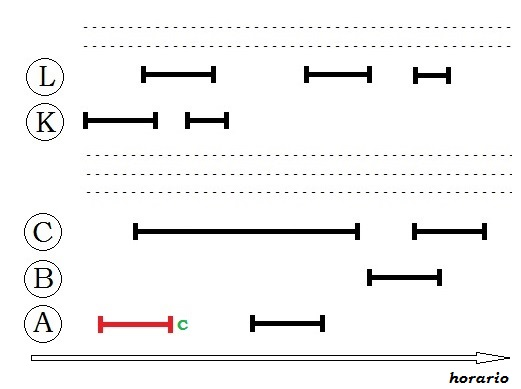
\includegraphics[scale=0.60]{imagenes/demo3.jpg}
	\end{center}
\end{figure}\\
Ahora, posicionados en C, realizar la búsqueda binaria de vuelos de salida de C hará que no consultemos vuelos que obviamente no podemos tomar (como el primer vuelo largo de C), haciendo que nos concentremos en el siguiente.
\begin{figure}[h]
	\begin{center}
	   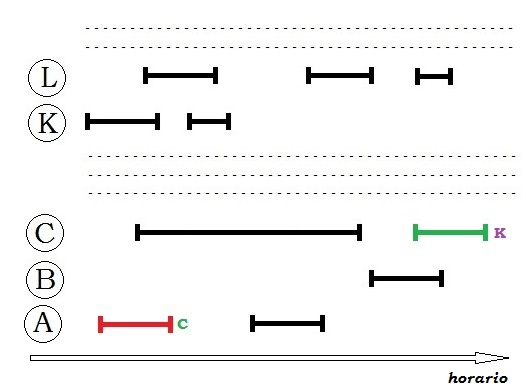
\includegraphics[scale=0.50]{imagenes/demo5.jpg}
	\end{center}
\end{figure}\\
Luego, dicho vuelos llevará nuestra atención a la ciudad K\\ Como nuestra busqueda binaria tiene 2 verificadores previos (explicado al inicio de la sección de complejidad), para el caso de ejemplo la búsqueda de vuelo se resuelve en O(1), viendo que no hay vuelos disponibles a la hora en la que llegamos a K.\\
Eso hace que volvamos a C para buscar otro vuelo, y a falta de otro para verificar, concluímos que a la hora de llegada a C (horario de llegada del primer vuelo de A) no es posible llegar hasta B (nuestro objetivo), por lo que guardamos en caché y procedemos a buscar otro vuelo en A.
\begin{figure}[h]
	\begin{center}
	   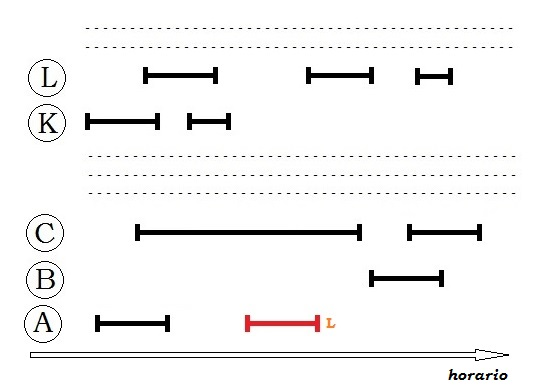
\includegraphics[scale=0.50]{imagenes/demo6.jpg}
	\end{center}
\end{figure}\\
Nuevamente, recursivamente llamamos a la ciudad J (ciudad disponible), y con búsqueda binaria, tomamos el primer vuelo posible.
\begin{figure}[h]
	\begin{center}
	   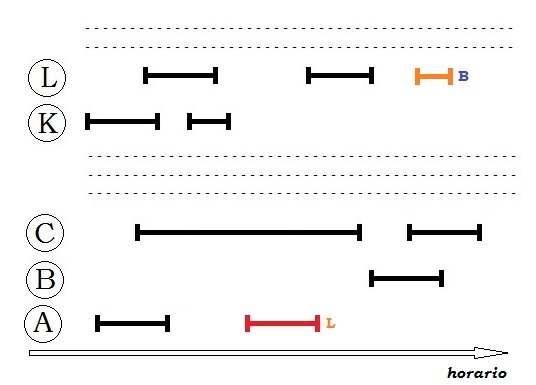
\includegraphics[scale=0.50]{imagenes/demo8.jpg}
	\end{center}
\end{figure}\\
Al tener ese vuelo como destino a B, guardamos en caché['L'] que desde L es posible llegar a B al horario de llegada del segundo vuelo de A, para no recalacularlo, y volvemos a A buscando otro vuelo que talvés nos termine llevando a B más temprano; como no lo hay, finaliza.

Si para el segundo vuelo de A, también hubieramos llegado a C, debido a que en cada ciudad se revisan los vuelos solo desde los que se pueden tomar hasta el ultimo sin revisar, \textbf{no hubieramos re-calculado el vuelo que se estaría tentado de calcular}, ya que la matriz caché indica que hay un calculo ya hecho a esa hora y simplemente basta con leerlo.\\
Ahora, si el segundo vuelo de A hubiera llegado lo suficientemente temprano como para tomar otro posible potencial vuelo de C,     caché['C'] \textit{pisaría} su valor para indicar la nueva franja horaria desde la que ya se conocen cálculos. 

Dicho eso, el peor de los casos, debido a sucesivos llamados recursivos podría acotarse superiormente por n búsquedas binarias, es decir, el peor caso del segundo submódulo tendría una cota superior \textbf{\textit{ O(n log n)}}.

\textit{\textbf{Notar que:}} la complejidad recién señalada, sugiere que se realizarían n búsquedas binarias (una por cada vuelo) de costo \textit{O(log n)} cada una, lo cual solamente pasaría si en todas las ciudades donde un vuelo llegara hubiera n vuelos de salida, lo cual es \textit{absurdo} ya que hay n vuelos en total y no hay vuelos que salgan y lleguen a la misma ciudad.\\
El único caso en el que se realizarían n búsquedas binarias sería que cada ciudad tenga solamente un vuelo de salida, pero, de darse ese caso, las mencionadas n búsquedas binarias se resolverían en O(1) cada una ya que el vector de vuelos de salida de cada ciudad tendría longitud = 1, resultando una complejidad \textit{O(n * 1) = O(n)}.\\
Por lo que \textit{\textbf{O(n log n)}} es una buena cota superior para el submódulo 2 de todo el programa.\\

\textit{\textbf{\underline{Análisis de mejor caso del submódulo 2}}}\\
Como el algoritmo se resuelve con la forma top-down, al comenzar mirando los vuelos de salida de A, esto hace que el mejor caso de este submódulo sea que \textbf{no salgan vuelos desde A}, teniendo una cota superior (de mejor caso) \textit{\textbf{O(1)}}.\\ \\

\noindent \underline{\textbf{\textit{Habiendo demostrado la complejidad de los 2 submódulos, la complejidad TOTAL del algoritmo es:}}} \\ \\
\textit{Complejidad submódulo 1 + Complejidad submódulo 2} = \\ \\
\textit{O(n log n) + O(n log n)} = \\ 

\noindent \textbf{\textit{O(n log n)}}\\ \\
\_\_\_\_\_\_\_\_\_\_\_\_\_\_\_\_\_\_\_\_\_\_\_\_\_\_\_\_\_\_\_\_\_\_\_\_\_\_\_\_\_\_\_\_\_\_\_\_\_\_\_\_\_\_\_\_\_\_\_\_\_\_\_\_\_\_\_\_\_\_\_\_\_\_\_\_\_\_\_\_\_\_\_\_\_\_\_\_\_\_\_\_\_\_\_\_\_\_\_\_\_\_\_\_\_\_\_\_\_\_\_\_\_\_\_\_\_\_\_\_\_\_\_\_\_\_\_\_\_\_\_\_\_\_\_\_\_\_\_\_\_
\\

\noindent \textit{\underline{\textbf{Demostración propiedad:}} Complejidad Ordenar subarreglos = Complejidad Ordenar arreglo entero}\\

\noindent \textbf{Sean} \textit{X,Y} y \textit{Z} arreglos tal que X.size() + Y.size() + Z.size() = n.\\
\textbf{Sea} \textit{tamI} el tamaño de un arreglo I. (Ej: tamX = X.size())\\
\textbf{Sea} sort() un algoritmo que ordena colecciónes tal que la complejidad de ordenamiento es O(coleccion.size() * log coleccion.size()) cuando el acceso a una posición de la colección se realiza en O(1).\\

\noindent Entonces, ordenar X, Y y Z con \textit{sort()} toma:

\indent \textit{\textbf{O(tamX * log tamX)}} + \textit{\textbf{O(tamY * log tamY)}} + \textit{\textbf{O(tamZ * log tamZ)}}\\

\noindent Como tamX + tamY + tamZ = n, entonces:

\indent (tamX * log tamX) \textless = (n * log n)\\
\indent (tamY * log tamY) \textless = (n * log n)\\
\indent (tamZ * log tamZ) \textless = (n * log n)\\

\noindent Luego, podemos acotar la complejidad mencionada anteriormente:

\indent \textit{\textbf{O(n log n)}} + \textit{\textbf{O(n log n)}} + \textit{\textbf{O(n log n)}} = \textit{3*\textbf{O(n log n) = O(n log n)}}\\

\noindent Quedando así demostrado que ordenar k subarreglos tal que la suma de sus longitudes es n, tiene una complejidad \textbf{O(n log n)}.

\newpage
\subsection{Experimentación}

\noindent Para el proceso de experimentación del problema se plantearon distintas pruebas para corroborar que el algoritmo propuesto funcionara correctamente, y que la cota de complejidad encontrada y justificada en la sección anterior, se cumpliera en la práctica.\\

\noindent Dado que el CPU de la computadora utilizada para tomar los tiempos no está atendiendo únicamente a nuestro proceso, realizar una sola vez cada prueba podría darnos valores que no son cercanos a los reales. Por lo tanto, para minimizar este margen de error, a cada prueba se la hizo ejecutar un total de 100 veces, y se tomó el mejor valor, es decir, el menor tiempo de ejecución obtenido. Notar que, tomar el mejor valor no es una mala decisión, ya que cuanto más chico sea el valor, más cerca estamos del valor real de tiempo que toma el algoritmo para una instancia dada.\\

\noindent En cada prueba, se tomaron métricas para la posterior evaluación del algoritmo en la práctica. Vale aclarar que la medición no contempla tiempos de salida de datos, sino que contempla:\\

\noindent \begin{enumerate}
\item La preparación de los datos de entrada para su procesamiento
\item El algoritmo que determina el mejor itinerario posible.\\
\end{enumerate}

\noindent Para el testeo, se diseñó un generador de instancias aleatorias que toma dos parámetros:\\


\noindent \begin{enumerate}
\item \textbf{Cantidad de ciudades:} determina cuántas ciudades se tomarán aleatoriamente que puedan ser origen o destino de los vuelos, seteando por lo menos un vuelo a cada una o desde cada una para que sean ciudades con sentido.

\item \textbf{La cantidad de vuelos presentes en la instancia}.\\
\end{enumerate}

\noindent Con este programa pudimos evaluar cuánto tiempo de ejecución toma nuestro algoritmo para distintas instancias aleatorias del problema.\\

\noindent Para todos los casos, se eligió una precisión de hasta 0,0001 ms (milisegundos). De ser menor, la tomamos como 0.\\

\noindent También desarrollamos un programa similar al explicado anteriormente, pero que arroja únicamente instancias de mejor caso.\\

\noindent Finalmente, el proceso de testing es:\\


\noindent \begin{enumerate}
\item Generación de instancia aleatoria, según parámetros prefijados.
\item Ejecución de dicha instancia 100 veces, tomando el mejor tiempo obtenido.
\item Repetición de los items 1 y 2 otras 99 veces y obtención del tiempo promedio.
\end{enumerate}

\noindent Con esta metodología de experimentación, realizamos pruebas en dos tipos de escenarios:\\
\noindent \begin{itemize}
\item Escenarios de casos aleatorios
\item Escenarios de mejor caso\\
\end{itemize}

\noindent A continuación, describiremos las particularidades de cada escenario.


\subsubsection{Escenarios de casos aleatorios}

\noindent En estos escenarios, decidimos evaluar casos aleatorios, generados por el generador de instancias aleatorias descripto anteriormente.\\

\noindent La idea fue tomar muestras del algoritmo haciendo variar la cantidad de vuelos, generando instancias que den origen y destino aleatorio a los mismos.\\

\noindent Para poder diferenciar bien los casos y poder analizar mejor, decidimos que cada escenario de las pruebas de caso aleatorio tenga una cantidad de ciudades constante. Esta capacidad de ciudades fue prefijada de manera que, si establecemos una cantidad m de ciudades, haya por lo menos un vuelo que salga o llegue a cada una, para que en la instancia haya por lo menos m ciudades activas.\\

\noindent A continuación, los gráficos resultantes de la experimentación en estos escenarios. Para los mismos, variamos la cantidad de vuelos aumentándolos de a 100 y elegimos probar con 20, 40 y 80 ciudades.\\

\noindent Para cada una de las pruebas, mostraremos la tabla con los valores obtenidos, los análisis de tiempos de ejecución y un análisis gráfico para estimar la complejidad del algoritmo.\\

\noindent \textit{Aclaración: Por simplicidad, nos referiremos de ahora en más con \textbf{n} a la \textbf{Cantidad de vuelos}. \\\\
}
	\begin{figure}[h]
		\begin{center}
		   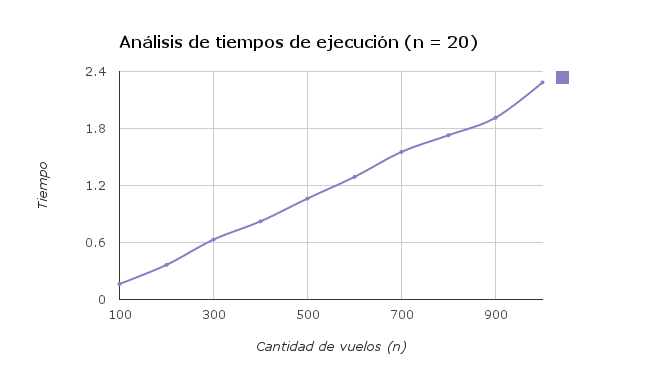
\includegraphics[scale=0.75]{graficos/tiempo_ejecucion20.png}
		\end{center}
	\end{figure}

\newpage
	\begin{figure}[h]
		\begin{center}
		   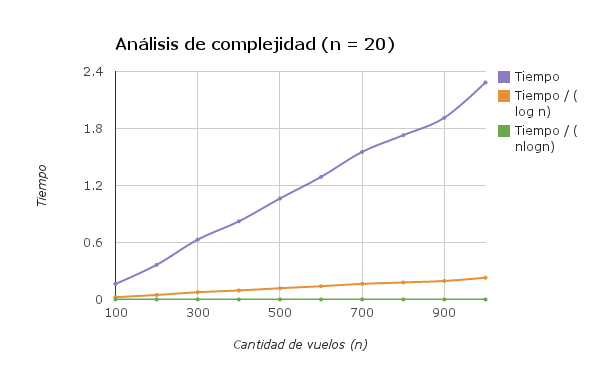
\includegraphics[scale=0.75]{graficos/complejidad_20.png}
		\end{center}
	\end{figure}



	\begin{figure}[h]
		\begin{center}
		    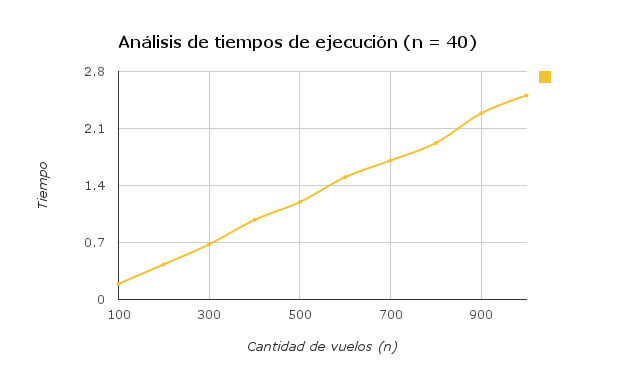
\includegraphics[scale=0.75]{graficos/tiempo_ejecucion40.png}
		\end{center}
	\end{figure}

\newpage


	\begin{figure}[h]
		\begin{center}
		   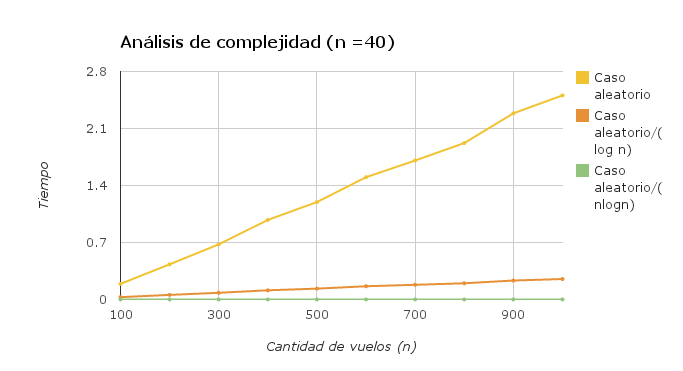
\includegraphics[scale=0.75]{graficos/complejidad_40.png}
		\end{center}
	\end{figure}


	\begin{figure}[h]
		\begin{center}
		   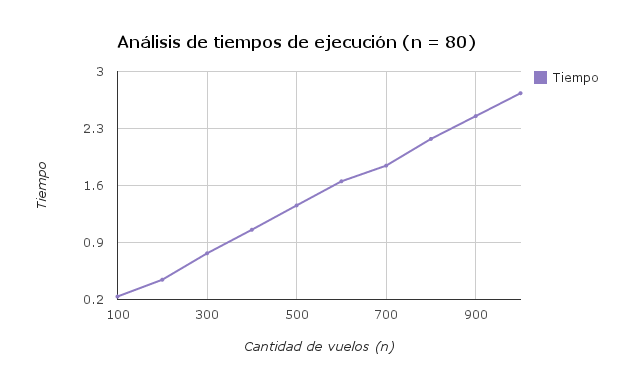
\includegraphics[scale=0.75]{graficos/tiempos_80.png}

		\end{center}
	\end{figure}

\newpage

	\begin{figure}[h]
		\begin{center}
		   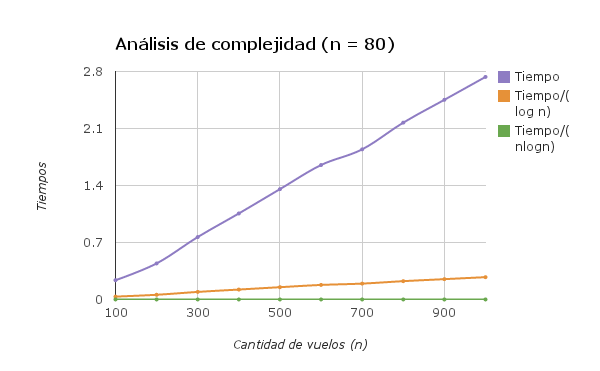
\includegraphics[scale=0.75]{graficos/complejidad_80.png}
		\end{center}
	\end{figure}

\subsubsection{Escenario de mejor caso}

\noindent En este escenario, realizamos una experimentación análoga a la detallada anteriormente: generamos instancias de mejor caso, haciendo variar la cantidad de vuelos aumentándolos de a 100, y dejando fija la cantidad de ciudades, de la misma forma en que se explicó en el escenario anterior. Sin embargo, en este caso, únicamente realizamos la experimentación considerando 40 ciudades. \\\\
	\begin{figure}[h]
		\begin{center}
		   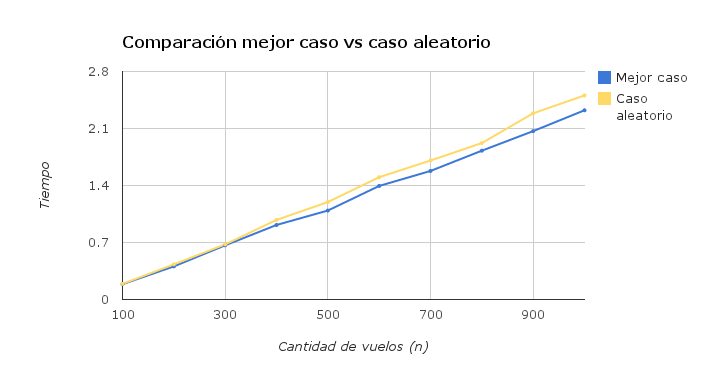
\includegraphics[scale=0.75]{graficos/comparacion_mejorcasoCasoAleatorio.png}
		\end{center}
	\end{figure}

\newpage
	\begin{figure}[h]
		\begin{center}
		   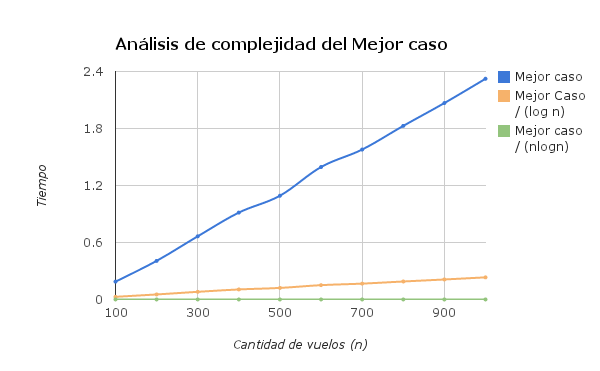
\includegraphics[scale=0.75]{graficos/complejidad_mejorCaso.png}
		\end{center}
	\end{figure}


\subsubsection{Conclusiones}
\textit{Aclaración: En esta sección continuamos refiriéndonos con \textbf{n} a la \textbf{Cantidad de vuelos}.}

\noindent Corroboramos lo analizado analíticamente, verificando en lo empírico que la complejidad del algoritmo propuesto es O(n log n).\\
\noindent En los gráficos de complejidad presentados en los distintos escenarios vemos claramente que al dividir punto f(n) de la función por log n nos queda una función lineal, y al hacerlo por n log n una constante. Esto solo podria pasar si efectivamente la curva que obtenemos al graficar los tiempos medidos está acotada por O(n log n).\\
\noindent Comprobamos además que a partir de la comparación de los gráficos obtenidos con instancias de 20, 40 y 80 ciudades, que la medición de tiempos, arroja para cualquiera de los tres escenarios curvas acotadas por O(n log n), por lo que corroboramos lo que analizamos desde lo analítico: la complejidad temporal del algoritmo no reside en la cantidad de ciudades que se usen para realizar los vuelos, si no en la cantidad de los mismos. Esto se debe a lo ya enunciado en el apartado de complejidad, donde expusimos que la cantidad de ciudades es del orden de n, ya que a lo sumo hay 2.n + 2 ciudades.\\
\noindent Por otro lado, en tanto al caso propuesto como mejor, observamos que arroja para cada n una medición de tiempo mejor que para una instancia de mismo n, pero de caso aleatorio. Sin embargo, este mejor caso solo impacta el cálculo de mejor camino, y no así la preparación de los datos, por ende esta curva obtenida a partir de la experimentación con instancias de mejor caso es también acotada por O(n log n), solo que con mejores tiempos debido a constantes de multiplicación menores.\\
\noindent De esta forma, corroboramos lo analizado analíticamente.\\

\end{document}